\documentclass[12pt]{article}

\usepackage{a4}
\usepackage{fullpage}
\usepackage[bahasa]{babel}
\usepackage{graphicx}
\usepackage[font=small,labelfont=bf]{caption}
\usepackage{parskip}

\setlength{\parskip}{1em}
\setlength{\parindent}{0em}
\tolerance 9999 \emergencystretch 3em\relax

\makeatletter
\newcommand{\chapterauthor}[1]{%
  {\parindent0pt\vspace*{-10pt}%
  \linespread{1.1}\small\scshape#1%
  \par\nobreak\vspace*{10pt}}
  \@afterheading%
}
\makeatother

\begin{document}
    \section*{Opini saya tentang Gugatan Perusahaan Media terhadap Layanan Siaran Langsung}
    \chapterauthor{ditulis oleh Rivo Juicer Wowor}

    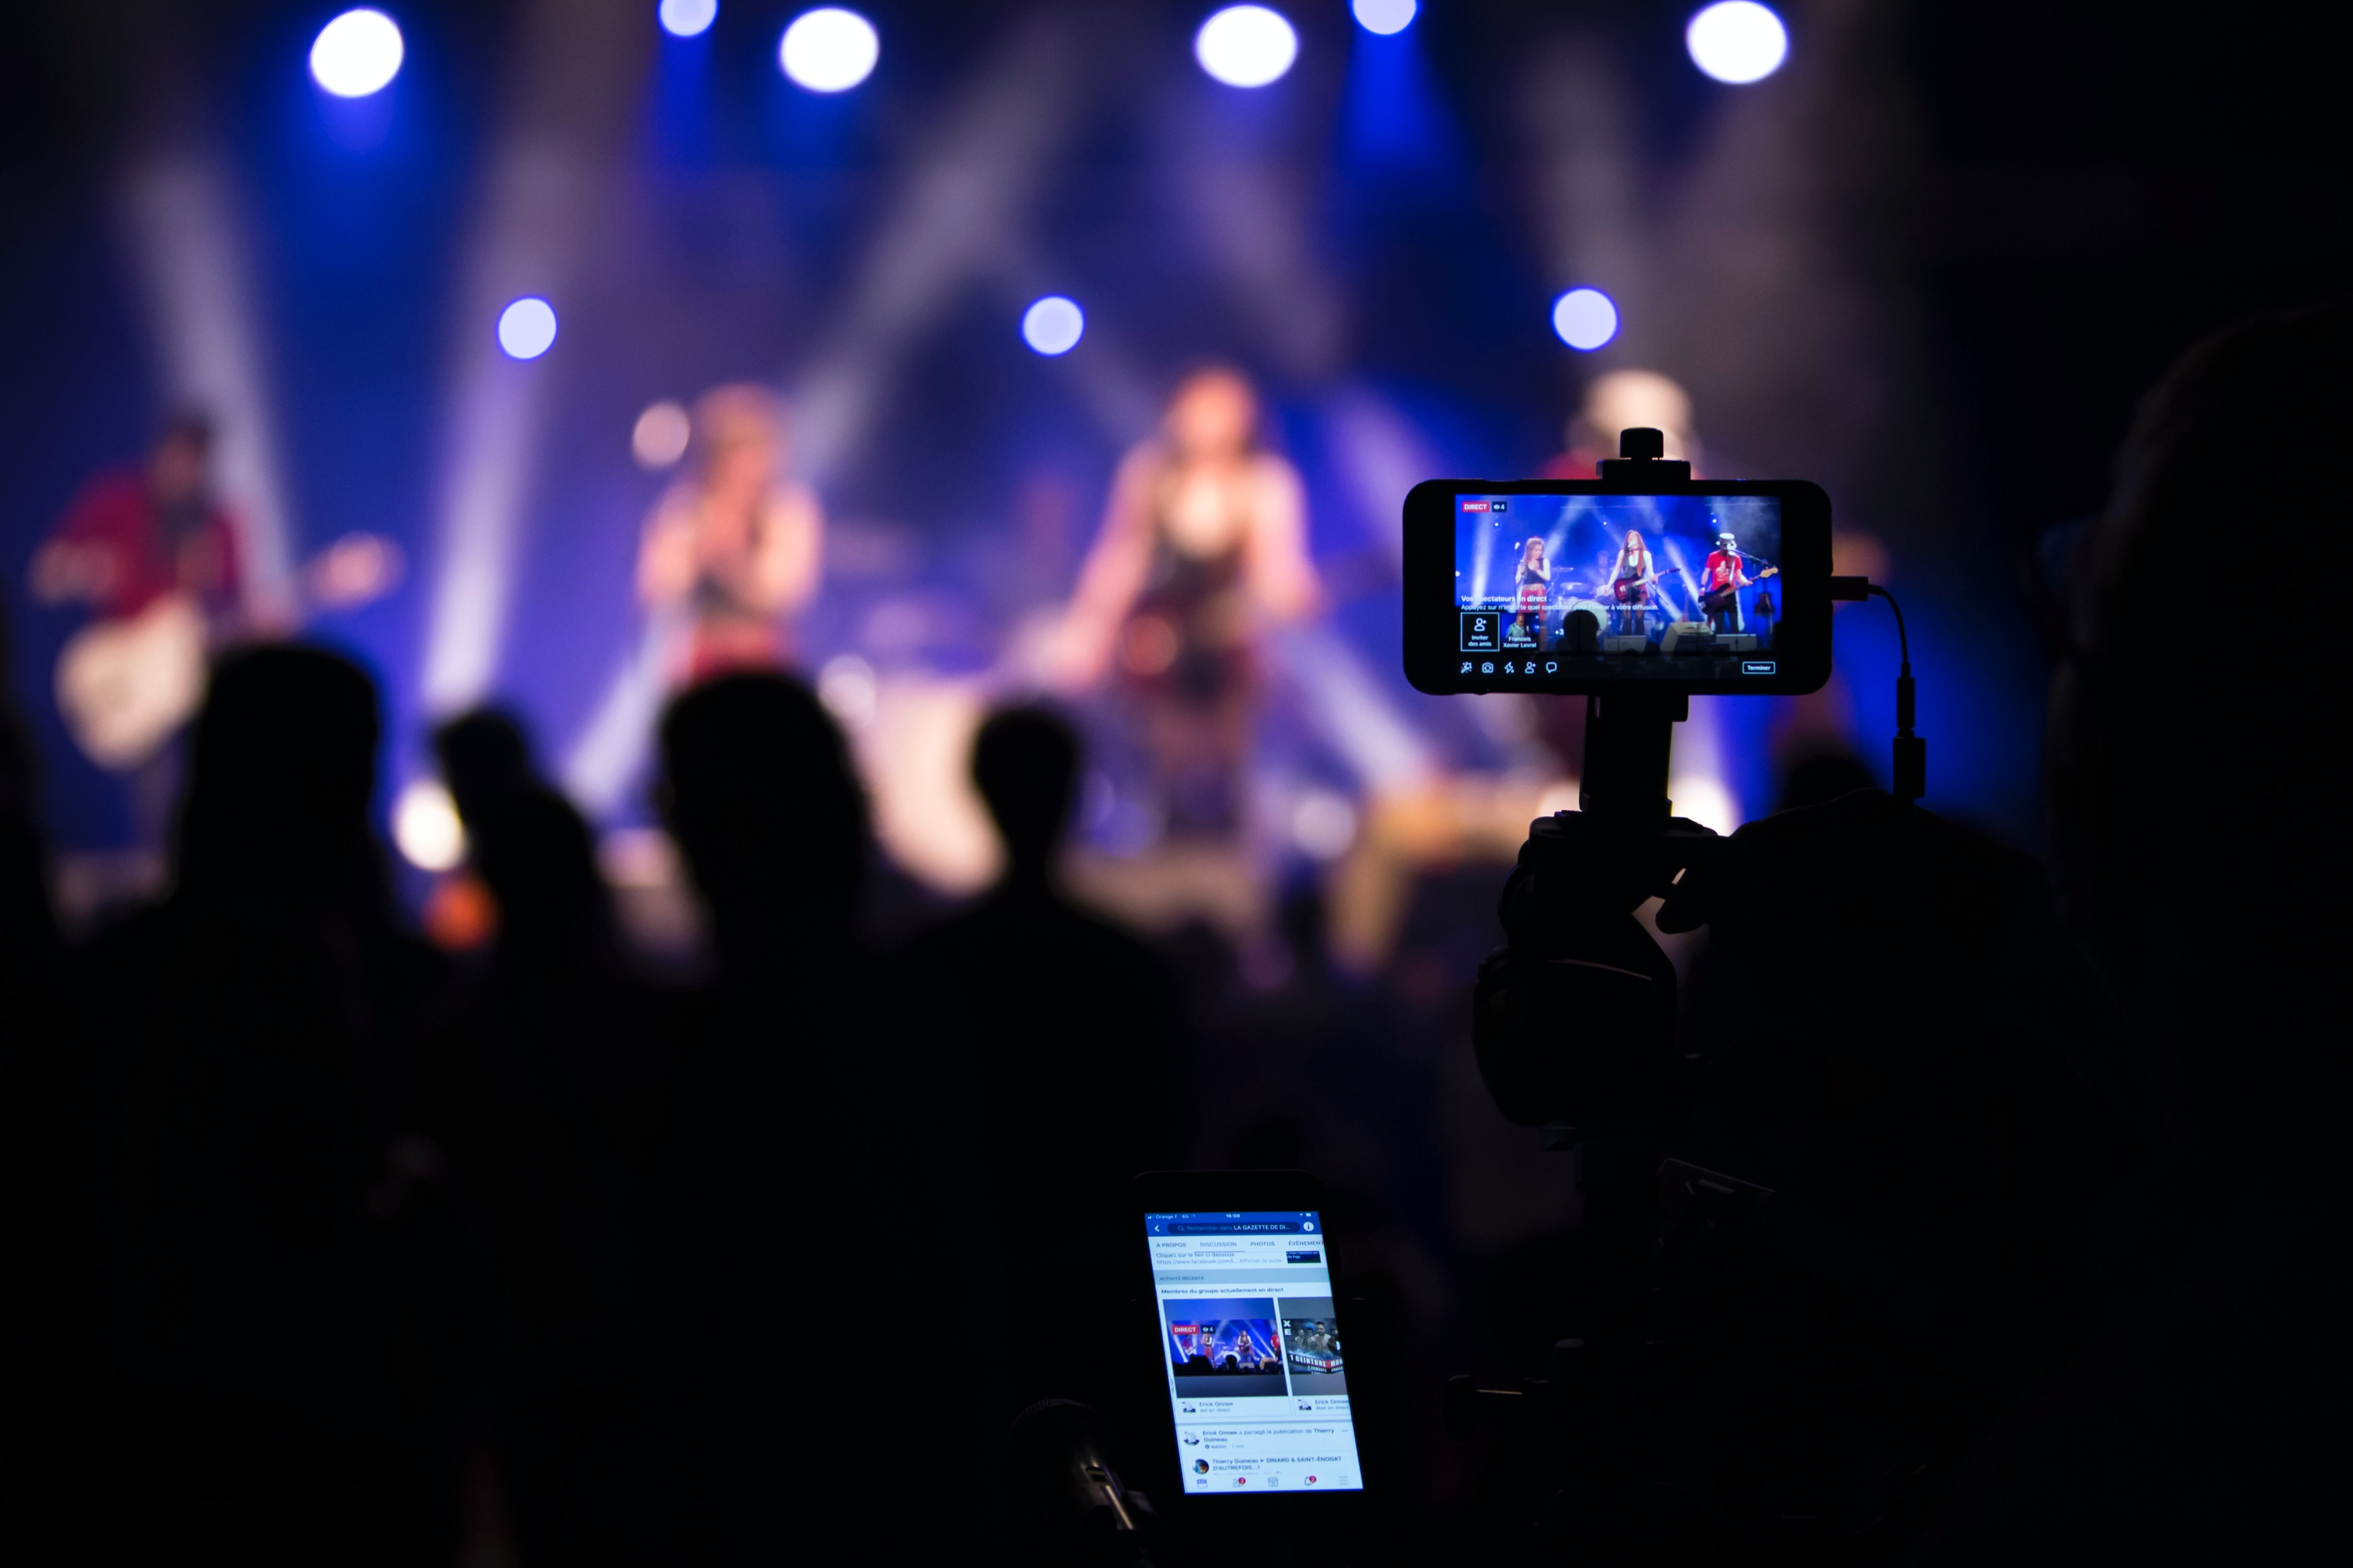
\includegraphics[width=1.0\textwidth,trim={0 17cm 0 0},clip]{images/livestream.jpg}
    \vspace{1pt}

    Pada bulan Agustus lalu, PT Visi Citra Mitra Mulia dan PT Rajawali Citra
    Televisi Indonesia menggugat UU Nomor 32 Tahun 2002 tentang Penyiaran ke
    Mahkamah Konstitusi.
    
    Kedua perusahaan media ini mengajukan uji materi
    soal UU Penyiaran dan menilai Pasal 1 angka 2 UU Penyiaran menyebabkan
    perlakuan berbeda antara penyelenggara penyiaran konvensional yang
    menggunakan frekuensi radio dengan penyelenggara penyiaran \emph{over
    the top (OTT)} yang menggunakan internet seperti \emph{YouTube} dan
    \emph{Netflix}. Jika gugatan ini dikabulkan, maka masyarakat baik
    perorangan maupun badan usaha terancam tidak leluasa menggunakan media
    sosial, seperti \emph{YouTube, Instagram, Facebook}, dan sebagainya
    untuk melakukan siaran langsung.
    
    Hal ini tentunya membuat banyak masyarakat yang emosi dan kecewa
    terhadap kedua perusahaan ini. Karena banyak orang yang menjadikan
    layanan ini sebagai sumber penghasilan bagi hidup mereka. Jika gugatan
    ini disetujui, maka otomatis sumber penghasilan mereka akan dipotong
    total serta menghambat pertumbuhan ekonomi kreatif dan digital di
    Indonesia. Selain itu, hak kebebasan berbicara juga akan dipertaruhkan
    disini. Karena layanan ini merupakan salah satu media masyarakat yang
    digunakan untuk mengekspresikan pendapat dan opini mereka.

    Gugatan ini juga dapat dibantahkan dengan pernyataan bahwa layanan
    siaran langsung seperti \emph{YouTube} dan lain-lain tunduk pada UU
    Telekomunikasi, bukan UU Penyiaran. Karena cara beroperasi layanan ini
    jauh berbeda dengan layanan televisi konvensional, meskipun keduanya
    sama-sama menggunakan audio dan visual sebagai medianya.

    Sebaiknya, layanan siaran langsung \emph{OTT} ini dilindungi oleh sebuah
    lembaga yang menaungi layanan media \emph{OTT} agar kegiatan siaran
    langsung dapat diawasi penggunaannya. Selain itu, undang-undang baru
    seharusnya dibuat untuk mengatur layanan siaran melalui internet. Agar
    layanan-layanan ini menjadi legal untuk dipakai di Indonesia. Karena
    jika gugatan seperti ini dikabulkan, maka akan sangat berdampak pada
    masa depan ekonomi kreatif Indonesia. Kita tidak tahu gugatan seperti
    apa lagi yang akan datang yang berkaitan dengan layanan Internet yang
    ada di Indonesia.
\end{document}